\chapter{Exoplaneter}
%
%
\begin{opgave}{Stjernernes spektre}{1} \label{opg:stjerners_spektre}
\opg For at se hvilke grundstoffer, der er i atmosfæren, skal du se for hvilke grundstoffer, der er absorptionslinjer. Vi kan derfor se, at der er eksempelvis er hydrogen, calcium og jern i atmosfæren.
\opg Generelt set er der mange flere absorptionslinjer for stjerner af type M end G. G0 og G5 er karakteriseret ved stærke Ca$^{2+}$-linjer, og svage til mellemstærke hydrogenlinjer, hvor Ca$^{2+}$-linjerne også ses i klasse M. Hydrogenlinjerne ses ikke på samme måde for M-stjernerne.
\opg Når en stjerne er kold, slås molekylerne ikke så let i stykker, og derfor kan vi finde molekyler som MgH og TiO i dens atmosfære. Dette skyldes, at varme hænger sammen med molekylernes kinetiske energi, hvorfor de intermolekylære kollisioner er voldsommere desto varmere stjernen er.  \\
Desuden ses absorptionslinjerne ikke når stofferne er så varme at de er ioniserede. \\
Der er dog ikke færre tunge stoffer i de varme, unge stjerner - tværtimod er der normalt flere. De gamle stjerner opstod nemlig dengang det interstellare medium ikke var lige så beriget med stoffer dannet i f.eks. supernovaer og kilonovaer.
\end{opgave}
%
%
\begin{opgave}{Planetkandidater}{1}
\opg Som udgangspunkt er det mest oplagt at lede efter stjernesystemer, der minder om vores eget Solsystem, da vi ved det giver de rette betingelser for liv som vi kender det. Solens spektralklasse er G, hvorfor det er mest oplagt at lede efter stjerner i denne spektralklasse og dem tæt på. Varmere stjerner giver ikke livet lang tid til at udvikle sig, og koldere har kraftige solvinde. Men det er selvfølgelig også spændende at analysere planeter om alle andre stjerner. 
\opg I figuren fra opgave \ref{opg:stjerners_spektre} ses det at spektraltyperne G0 og G5 er karakteriseret ved bl.a. stærke Ca$^{2+}$-linjer og svage til mellemstærke hydrogenlinjer. Derudover adskiller de sig også fra K og M ved fraværret af linjer for metaller som Fe, Mg og Ti. De varmeste stjerner har kraftige hydrogenlinjer, så dem kan man prøve at undgå. Desuden kan man kigge på spektrets samlede form og se hvor dets toppunkt ligger.
\end{opgave}
%
%
\begin{opgave}{Stjernespektrer og temperaturer}{1}
\opg Benyttes Wiens forskydningslov med temperaturene $\SI{5500}{\kelvin} \leq T \leq \SI{6000}{\kelvin}$, idet Solen ligger i det temperaturinterval, fås
\begin{align*}
    \SI{483}{\nano\metre} \leq \lambda_\text{max} \leq \SI{527}{\nano\metre}
\end{align*}
Det præcise tal er ikke vigtigt, men det skal gerne fremkomme at tallet skal være omkring $\sim\SI{500}{\nano\metre}$. Intervallets størrelse afhænger af hvor optimistisk man er på livets vegne.
\opg Lys med bølgelængde omkring \SI{500}{\nano\metre} ses af mennesker som værende et sted mellem blå og grøn. Solen ser dog ikke grøn ud grundet dens andre bølgelængder og hvordan det menneskelige øje fungerer.
\end{opgave}
%
%
\begin{opgave}{Jævn cirkelbevægelse}{1}
\opg En jævn cirkelbevægelse er en idealiseret bevægelsesform, hvor et legeme bevæger sig i en bane formet som en perfekt cirkel, hvor farten (og afstanden) er den samme hele vejen rundt. Hastigheden ændrer sig dog, da bevægelsesretningen ændres (derfor må der ske en acceleration, og den peger indad mod centrum).
\opg Perioden er defineret som den tid det tager at bevæge sig en omgang, hvilket kan skrives som
\begin{align*}
    P = \frac{x}{v} \: ,
\end{align*}
hvor $v$ er farten og $x$ er den i omløbet tilbagte distance. Eftersom den tilbagelagte distance er en cirkel med radius $r$, så er
\begin{align*}
    x = 2\pi r \: ,
\end{align*}
hvorved
\begin{align*}
    P = \frac{2\pi r}{v}
\end{align*}
\opg Jordens afstand til Solen er nogenlunde $r_\oplus = \SI{1.0}{AU}$ og perioden er $\SI{1.0}{yr}$. Dermed bliver Jordens banehastighed under antagelse af jævn cirkelbevægelse
\begin{align*}
    v = \frac{2\pi r_\oplus}{P_\oplus} = \frac{2\pi\cdot\SI{1.0}{AU}}{\SI{1.0}{yr}} = \frac{2\pi\cdot\SI{1.496e11}{\metre}}{\SI{3.156e7}{\second}} = \SI{29.8}{\kilo\metre\per\second}
\end{align*}
Bruger man approksimationen at $\SI{1.0}{yr} \simeq \SI{\pi e7}{\second}$ fås
\begin{align*}
    v = \frac{2\pi r_\oplus}{P_\oplus} \simeq \frac{2\pi\cdot\SI{1.0}{AU}}{\SI{\pi e7}{\second}} = \frac{\SI{2}{AU}}{\SI{1e7}{\second}} = \SI{2e-7}{AU\per\second} = \SI{29.9}{\kilo\metre\per\second}
\end{align*}
\end{opgave}
%
%
\begin{opgave}{Den Beboelige Zone}{1}
Afstanden isoleres i ligning \ref{k-eq:PlanetTemperatur} i kompendiet:
\begin{align*}
    T_p = T_\star\left(\frac{1-A}{4}\right)^{1/4}\left(\frac{R_\star}{r}\right)^{1/2} \;\Rightarrow\; rT_p^2 = T_\star^2\left(\frac{1-A}{4}\right)^{1/2}R_\star \;\Rightarrow\; r = R_\star\left(\frac{T_\star}{T_p}\right)^2 \left(\frac{1-A}{4}\right)^{1/2}
\end{align*}
\opg Nu bestemmes $r$ for temperaturene $T_p = \SIrange{273.15}{373.15}{\kelvin}$
\begin{align*}
    \mathrm{a) } \quad &T_\star = T_\odot, \: R_\star = R_\odot \: \Rightarrow \: r_\textsc{bz} = \SIrange{6,9e10}{12,9e10}{\metre} = \SIrange{,46}{,86}{AU} \\
    \mathrm{b)} \quad &T_\star = 2T_\odot, \: R_\star = R_\odot \: \Rightarrow \: r_\textsc{bz} = \SIrange{2.77e11}{12,9e10}{\metre} = \SIrange{1.85}{3.46}{AU} \\
    \mathrm{c)} \quad &T_\star = T_\odot, \: 5R_\star = R_\odot \: \Rightarrow \: r_\textsc{bz} = \SIrange{3.47e11}{6.47e11}{\metre} = \SIrange{2.32}{4.32}{AU} \\    
\end{align*}
\opg Afstanden mellem Jorden og Solen er \SI{1}{AU}, hvilket er udenfor den estimerede beboelige zone. Dette betyder at Jorden ikke opfylder antagelserne som ligning \ref{k-eq:PlanetTemperatur} bygger på, fordi Jorden har en varm jernkerne, som gør at Jorden ikke er i termisk ligevægt. Ofte estimerer man dog zonen antaget en jordlignende planet. Det er i det hele taget en kompliceret sag, og normalt antages Jorden at ligge i den indre kant af den beboelige zone om Solen. Desuden burde man ændre på stjernens temperatur, når man ændrer radius og vice verca, antaget at den er i ligevægt. 
\end{opgave}
%
%
\begin{opgave}{Gravitationslinser}{1}
I afsnit \ref{k-sec:GravLinse} i kompendiet om gravitationslinsemetode blev det nævnt at begivenheden skal observeres af flere forskellige målinger.
\opg Kigges der ud i verdensrummet er der mange ting der kan ses. En lyskurve, som beskrevet i afsnittet, kan også skyldes andre fænomener, en fejl i målingerne, eller bare et statistisk udsving. Flere målinger kan være med til at øge den samlede sandsynlighed for at der faktisk er en planet. Man vil typisk sætte et krav som fx at signalet fra planeten skal være 5 gange stærkere end støjen, når man kombinerer dataen. Det kan også opnå med en enkelt måling, men det er sværere. %For at man kan konkludere noget naturvidenskabeligt, så er man derfor nød til at observere det samme fænomen på en sådan måde, sådan så der kun er en realistisk konklusion.
\opg Gravitationslinsemetoden kræver en meget specifik situation, netop at en stjerne med tilhørende planet bevæger sig ind foran en anden stjerne langs Jordens synslinje. %For at "lensingen"\;kan ske er de to stjerner separeret af en anseelig afstand, hvorfor de ikke nødvendigvis påvirker hinanden gravitationelt signifikant. 
Det er derfor meget muligt at begivenheden kun forekommer én gang. %, og hvis den ene stjerne er i bane om den anden, så er perioden så kæmpe stor at det er urealistisk at vente lang nok tid til at se det igen. Perioden er så stor grundet Keplers 3. lov, $P^2 \propto a^3$, hvor $a$ er den halve storakse for ellipsebanen, hvilket nogenlunde er i samme størrelsesorden som afstanden mellem lyskilden og planetsystemet, som jo er stor på astronomisk skala.
\opg Hvis man kun har ét tidsrum til at observere begivenheden, og vil optimere sandsynligheden for at signalet er en planet (eller vise det ikke er), så må man tage gode målinger mens man kan. Det kan gøres ved ideelt at observere begivenheden med forskelligt udstyr. På den måde får man et stort nok datasæt selvom tidsperioden er kort.
%men stadig vil kunne afvise, at det er er andet end en planet, så er man for det første nødt til at have så mange målinger med forskelligt udstyr, at man kan afvise at der er tale om en fejl i målingerne eller en statistisk afvigelse fra normen. Derudover er man også nød til på en eller anden måde at kunne verificere at det ikke kan skyldes andre fænomener. Den bedste måde at gøre dette på, er at observere systemet i før og efter, med flere forskellige instrumenter, så man ved hvordan området på stjernehimlen normalt ser ud.
\end{opgave}
%
%
\begin{opgave}{Estimat af planetmasse}{2}
Til dette benyttes ligningerne \eqref{k-rvstang} og \eqref{k-eq:K3Fancy} i kompendiet. Først indsættes ligning \eqref{k-rvstang} i ligning \eqref{k-eq:K3Fancy}
\begin{align*}
	\frac{4\pi^2}{G(M_p+M_\star )} &= \left(\frac{2\pi r_\star \sin(i)}{v_{||}}\right)^3\left(P_\star r^3\right)^{-1} \\
	\implies \frac{4\pi^2}{G(M_p+M_\star )} &= \left(\frac{2\pi r_\star \sin(i)}{v_{||}}\right)^3\left(P_\star r_\star ^3\left(\frac{M_\star  + M_p}{M_p}\right)^3\right)^{-1}\; .
\end{align*}
Herefter er det "bare"\;oprydning, hvor det første der gøres er at skrive det hele ud ved at opløse parenteserne
\begin{align*}
	\frac{4\pi^2}{G(M_p+M_\star )} = \frac{8\pi^3 r_\star^3 \sin^3(i)}{v_{||}^3} \frac{M_p^3}{P_\star r_\star ^3(M_\star  + M_p)^3} \; .
\end{align*}
Så forkortes ting ud
\begin{align*}
	\frac{1}{G} = \frac{2\pi \sin^3(i)}{v_{||}^3} \frac{M_p^3}{P_\star (M_\star  + M_p)^2} \; ,
\end{align*}
og slutteligt isoleres $M_p^3\sin^3i$ for at opnå resultatet
\begin{align*}
	M_p^3\sin^3(i) = \frac{P_\star v_{||}^3 (M_\star  + M_p)^2}{2\pi G} \; .
\end{align*}
\end{opgave}
%
%
\begin{opgave}{Overfladetemperatur på planeter}{2}
\opg For at kunne komme frem til udtrykket starter vi med at se på fluxen, altså det lys, som vi modtager. Fluxen er givet ved
 \begin{align*}
 F &= \frac{L_\star}{4\pi D^2} = \frac{4\pi R_\star^2 \sigma T_\star^4}{4\pi D^2} = \left( \frac{R_\star}{D}\right) ^2 \sigma T_\star^4 \: .
 \end{align*}
 Vi ser nu på den energi som planeten absorberer. Vi antager at vi har en jævn kugle, som energien fordeles jævnt udover. Derudover skal vi have albedoen i spil, i det den fortæller os hvor meget lys, der bliver reflekteret. 
 \begin{align*}
 L_\text{abs} &= \pi R_{p}^2 F \left( 1-A\right) = \pi R_{p}^2 \left( \frac{R_\star}{D}\right) ^2 \sigma T_\star^4 \left( 1-A\right) = \frac{\pi R_p^2R_\odot^2 \sigma T_\star^4}{d^2} \left( 1-A\right) \: .
 \end{align*}
\opg Termisk ligevægt betyder at temperaturen er konstant. Derfor er mængden af termisk energi (varme), planeten optager fra sine omgivelser, den samme som mængde af termisk energi, den afgiver til omgivelserne.
\opg Idet planeten er antaget som værende et sortlegeme er
\begin{align*}
 L_\text{uds} = 4\pi R_p^2 \sigma T_p^4 \: .
 \end{align*}
Planeten er også i termisk ligevægt, hvorfor den udsender lige så meget energi, som den absorberer. 
 \begin{align*}
 L_\text{uds} &= L_\text{abs} \\
 \Rightarrow 4\pi R_m^2 \sigma T_m^4 &= \frac{\pi R_m^2R_\odot^2 \sigma T_\odot^4}{d^2} \left( 1-A\right) \\
 \Rightarrow 4T_m^4 &= \left( \frac{R_\odot}{d} \right) ^2 T_\odot^4 \left( 1-A\right) \\
 \Rightarrow T_m^4 &= \left( \frac{R_\odot}{d} \right) ^2 \frac{\left( 1-A\right)}{4} T_\odot^4\\ 
 \Rightarrow T_m &= \left( \frac{R_\odot}{d} \right) ^{1/2} \left( \frac{\left( 1-A \right) }{4} \right) ^{1/4} T_\odot
 \end{align*}
 \opg Vi bruger udtrykket, som vi lige har fundet og bestemmer temperaturen på overfladen. 
 \begin{align*}
 T_p \approx \SI{40}{\kelvin} \: .
 \end{align*}
 Vi antager at den roterer hurtigt. Det har den betydning, at vi antager at temperaturen er den samme på over det hele, der vil altså ikke være noget "dag og nat". Den teoretiske værdi siger \SI{40}{\kelvin} og temperaturen er blevet vurderet til \SI{65}{\kelvin}. Det tyder derfor på, at vores antagelse om hurtigt rotation muligvis ikke er så god. Hvis den roterer langsomt, vil det betyde at temperaturen ikke er den samme overalt, hvilket kan forklare hvorfor temperaturen er blevet vurderet til \SI{65}{\kelvin}. %Kilde?
\end{opgave}
%
%
\begin{opgave}{Spektre af planetatmosfærer}{2}
\opg Absorptionslinjerne fra OH-grupper og ketoner er meget karakteristiske for hvor i spektret de ligger. Specielt OH-grupper da linjen er ekstremt bred og næsten ligner en parabel. Eftersom vand har to O-H-bindinger vil vand give en meget kraftig linje, der vil ligne en alkohol, men den ville kunne kendes fra andre alkoholer ved det komplette fraværd af linjer fra C-H-bindinger. Vand er en ekstremt vigtig biomarkør, og kan vand ses i spektret fra en planets atomsfære er det en meget værdifuld information. Ketonlinjen vil kunne ses i eksempelvis CO$_2$, og den vil kunne kendes fra andre ketoner ved manglen på C-H-bindinger. Carbondioxid er også en vigtig biomarkør, hvorfor dette er af interesse. Carboxylsyren er ikke en ligeså vigtig biomarkør, men den vil dog være meget karakteristisk i spektret, idet man vil se en karakteristisk linje for C=O-bindingen og en karakteristisk linje fra O-H-bindingen. Yderligere vil OH-linjen være meget markant forskudt, sammenlignet med dens placering, hvis den ikke havde været i nærheden af ketonen. Grunden til at carboxylsyren er så karakteristisk er at oxygen er et meget elektrontiltrækkende atom, hvorfor de to O'er vil "trække"\:meget i det enlige carbons elektroner. Denne polarisering af bindingerne påvirker spektret idet det ændrer på energien i bindingen. Denne ændring er meget svær at beskrive, da den afhænger af mange faktorer, og det er også derfor de forskellige funktionelle gruppers absorptionslinjer kan være så relativt mange forskellige steder.
\opg Den største udfordring er, at man er nødt til at kende et absorptionsspektrum fra planetens atmosfære, og sikre sig at det faktisk er det man har målt på. Det er beskrevet i kompendiet, hvordan dette i grove træk kan lade sig gøre. Spektret vil også være Dobblerforskudt og på andre måder forstyrret, hvorfor der er en masse bearbejdning inden man overhovedet kan gå i gang med at fortolke spektret. Fx kan dele af lyset være absorberet af gas på dets rejse mod Jorden. Det næste problem er, at hele spektret kommer samtidig. Det spektrum man ser, er resultatet af alle absorptionerne fra alle atomer og molekyler i atmosfæren, hvilket gør spektret meget mere komplekst. Godt nok er en alkohol eller carboxylsyre meget karakteristisk i IR-spektret fra en prøve af et enkelt stof i kemilaboratoriet på Jorden, men hvis spektret består af absorptioner fra mange forskellige molekyler, risikerer man at opløsningen ikke er god nok til at skelne linjerne fra hinanden. Linjerne har en bredde grundet bl.a. forskellige hastigheder af molekylerne, så de Dopplerforskydes lidt forskelligt. 
%Det kunne eksempelvis være at en linje ligner den fra en keton, men i virkeligheden bare er resultatet af mange forskellige linjer, der ligger oveni hinanden. Har man ikke andet en spektret fra en planets atmosfære er det derfor meget komplekst at konkludere noget mere specifikt end eksempelvis "spektret tyder på at planetens atmosfære indeholder vand, idet eksistensen af van forklarer dele af spektret".
\end{opgave}
%
%
\begin{opgave}{Atmosfærekrav}{3}
For at en planet kan have en stabil atmosfære er den nød til at kunne holde simple molekyler fanget i dens tyngdefelt. Massen af $O_2$ er $m_{O_2} = \SI{5,31e-26}{\kilo\gram}$.
\opg Newtons gravitationslov siger at tyngdekraften mellem legemer i afstand $r$ er
\begin{align*}
	F_G = G\frac{mM}{r^2} \: .
\end{align*}
Bruges Newtons anden lov er
\begin{align*}
	mg &= G\frac{mM}{r^2} \: , \\
	g &= G\frac{M}{r^2} \: ,
\end{align*}
hvor $g$ er tyngdeaccelerationen.
\opg Fra mekanik er de omtalte energier
\begin{align*}
	K &= \frac{1}{2}mv^2 \: , \\
	V &= mgh \: ,
\end{align*}
hvor $h$ er afstanden fra nulpunktet. Defineres planetens centrum som nulpunktet er $h = R_p$, og sættes de to energi lig hinanden fås
\begin{align*}
	\frac{1}{2}mv^2 = mgR_p \: .
\end{align*}
Isoleres $v^2$ før tyngdeaccelerationen fra før indsættes, fås
\begin{align*}
	v_\mathrm{ecs}^2 = \frac{2M_pG}{R_p} \: .
\end{align*}
\opg I ligningen fra kinetisk gasteori isoleres $v_{av}^2/2$
\begin{align*}
	\frac{1}{2}v_{av}^2 = \frac{3}{2}\frac{k_BT}{m} \: .
\end{align*}
Kombineres dette med undvigelseshastigheden fås
\begin{align*}
	\frac{3}{2}\frac{k_BT}{m} &= \frac{M_pG}{R_p} \\
	\implies \frac{M_p}{R_p} &= \frac{3}{2}\frac{k_BT}{mG} \: .
\end{align*}
\opg Udtrykket på venstre side af lighedstegnet er egenskaber ved selve planten, mens udtrykket på højre side er egenskaber ved plantens atmosfære, der udtrykker partiklerne i atmosfærens hastighed. Hvis planeten skal kunne fastholde atmosfæren må den hastighed ikke overskride undvigelseshastigheden, hvorfor uligheden må være
\begin{align}
	\frac{M_p}{R_p} > \frac{3}{2}\frac{k_BT}{m_{O_2}G} \: .
\end{align}
\opg For Jorden er forholdet mellem masse og radius
\begin{align*}
	\frac{M_\oplus}{R_\oplus} = \frac{\SI{5,972e24}{\kilo\gram}}{\SI{6371}{\metre}} = \SI{9.3737e+17}{\kilo\gram\per\metre} \: .
\end{align*}
Sættes tallene ind i højresiden fås
\begin{align*}
	\frac{3}{2}\frac{k_BT}{m_{O_2}G} &= \frac{3\cdot\SI{1.38065e-23}{\joule\per\kelvin}\cdot(273,15 + 16)\SI{}{\kelvin}}{2\cdot\SI{5,31e-26}{\kilo\gram}\cdot\SI{6.6742e-11}{\metre\cubed\per\kilo\gram\per\second\squared}} = \SI{1.6886e+15}{\kilo\gram\per\metre} \: .
\end{align*}
Ergo er ligningen opfyldt for Jorden.
\end{opgave}
%
%
\begin{opgave}{Bose-Einstein kondensat og laserkøling}{2}
\opg $E = \frac{hc}{\lambda}$ hvor $h$ og $c$ er konstanter, hvorfor energien bliver større, hvis bølgelængden bliver kortere.
\opg Ingenting, da atomets energiniveauer er kvantiseret, hvorfor der ikke kan ske noget, hvis ikke fotonens energi er lige præcis nok til at flytte elektronen fra ét energiniveau til et andet - medmindre energien er høj nok til at frigøre elektronen helt og dermed ionisere atomet.
\opg For at holde styr på atomerne kaldes den der bevæger sig mod laseren (1), og den der bevæger sig væk fra (2). Kaldes retningen af atom (1) for den positive retning, gælder følgende: \\
(1) Laseren bevæger sig mod atomet, og altså i negativ  retning. \\
(2) Laseren bevæger sig væk fra atomet, og altså i positiv retning.
\opg Der kigges nu på samme foton fra de to referencesystemer. \\
(1) Fotonen er udsendt fra en kilde, der bevæger sig mod atomet, hvorfor fotonen er blåforskydt. \\
(2) Fotonen er udsendt fra en kilde, der bevæger sig væk fra atomet, hvorfor fotonen er rødforskydt.
\opg De to atomer ser ikke fotonen, som havende samme bølgelængde, og dermed ikke samme energi. Da atomerne er ens, har de samme energiniveauer, men da atomerne oplever fotonen forskelligt, så passer fotonen ikke med en overgang i begge atomer.
\opg Atomet skal gerne holdes samlet i midten af den fælde, hvori de holdes. De atomer, der bevæger sig væk fra fælden mod laseren ser laseren som blåforskudt. Vælges laseren til at have en bølgelængde, der er lidt længere end den, der svarer til overgangen hvis atomet står stille, kan kun atomer på vej ud af fælden mod laseren opleve lyset, som værende Dopplerforskudt på den måde, der gør det muligt for atomet at interagere med lyset. Derved kan man sikre sig at man kun påvirker de rigtige atomer, og derved køler gassen.
\opg Dette kan opgavens forfatter ikke besvare. Ifølge JR er svaret entydigt "ja"!
\end{opgave}
%
%
\begin{figure}
	\centering
	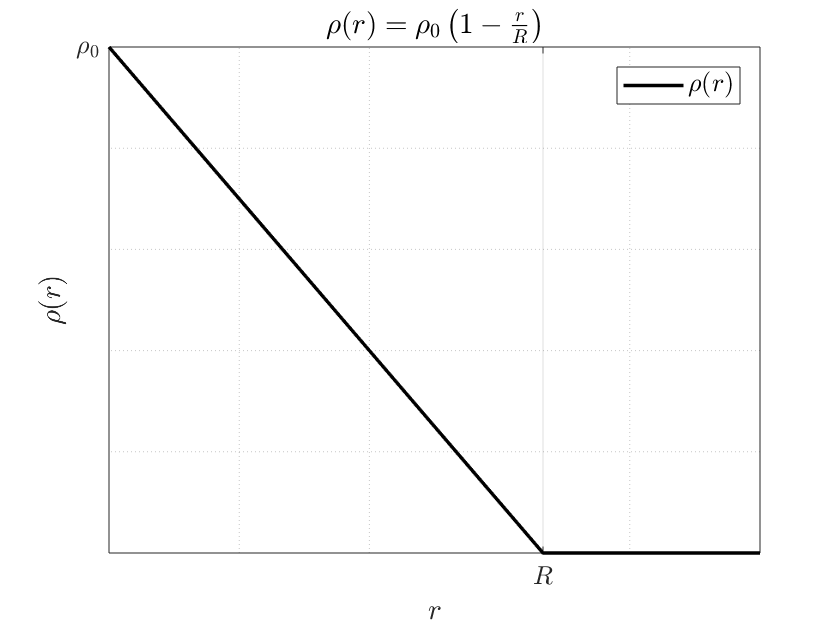
\includegraphics[width=.6\textwidth]{Astrofysik/billeder/PlanetMasse.png}
	\caption{Tegning af funktionen $\rho(r)$ for $r\geq0$.}
	\label{fig:PlanetMasse}
\end{figure}
%
%
\begin{opgave}{Masse af en planet}{2}
\opg Se figur \ref{fig:PlanetMasse}.
\opg Funktionen indsættes i integralet, som derefter løses
\begin{align*}
    M = 4\pi\int_0^R\rho(r)r^2\d r = 4\pi\rho_0\int_0^R r^2 - \frac{r^3}{R} \d r = 4\pi\rho_0 \left[\frac{1}{3}r^3 - \frac{r^4}{4R}\right]_0^R = 4\pi\rho_0 \left[\frac{1}{3}R^3 - \frac{1}{4}R^3\right] = \frac{1}{3}\pi\rho_0R^3 \: .
\end{align*}
\end{opgave}
%
%
\begin{opgave}{Tyngdeaccelerationen indeni en planet}{3}
\opg Densitet har enheden \si{\kilo\gram\per\metre\cubed}, mens $r$ har enheden \si{\metre}, hvorfor
\begin{align*}
    [A] = [\rho r^2] = \si{\kilo\gram\per\metre} \: .
\end{align*}
\opg For at forstå sådanne funktioner kan det være værd at kigge på hvilket dele af funktionen, der er størst i hvilke områder: \\
-- \; $\lim\limits_{r\rightarrow0}(1/r^2) = \infty$, mens $\exp(-R/c) < \infty$, hvorfor $1/r^2$ dominerer for små $r$. Ergo opfører $\rho(r)$ sig som $1/r^2$ for små værdier af $r$. \\
-- \; Eksponentialfunktionen er aftagende idet eksponenten er negativt på hele definitionsmængden, hvorfor den kun bliver dominerende, hvis den aftager tilpas meget langsommere end $1/r^2$. Jo mindre $c$ bliver, desto større bliver $(r-R)/c$, hvorfor eksponentialfunktionen dominerer mest for små værdier af $c$. Eksponenten går mod 0, for $r \rightarrow R$ uanset hvad $c$ er, hvorfor betydningen af $c$ må blive mindre jo større $r$ bliver. \\
-- \; Planetens radius er $R$, hvorfor $\rho(r) = 0$ for $r>R$, hvilket ses ved at funktionen brat går i nul og bliver der. \\
-- \; Af figurens ses det at $\rho(r) \xrightarrow{r\rightarrow0} \infty$ uanset hvad værdien af $c$ er. \\
-- \; Det ses også at $\rho(r)$ først begynder at afvige drastisk fra $1/r^2$, når $c<0,5$. For alle værdier af $c$ bliver grafen godt nok næsten flad eller voksende når $r$ nærmer sig $R$, men det sker meget sent for de største værdier af $c$. \\
-- \; For de mindste værdier af $c$ bliver eksponenten så stor at den meget hurtigt begynder at dominere, hvorfor $1/r^2$ delen kun ses for meget små $r$. \\ \\
-- \; Alt i alt er størstedelen af planetens masse samlet tæt på centrum, og interessant nok er der ikke ret meget masse omkring $r = R/2$, hvis $c$ er tilpas lille. \\
-- \; Hvorvidt denne funktion overhoved kan modellere massen af en planet skal være usagt, men som teoretisk eksempel er den ganske interessant.
\opg Det er bare integralets grænse, der skal ændres, og formelt set bør man også ændre integrationsvariablen så
\begin{align*}
    M(r) = \int_0^r\rho(r')4\pi (r')^2\d r' \: .
\end{align*}
\opg Nu er det bare at kombinere formlerne og løse integralet.
\begin{align*}
    g(r) &= \frac{G}{r^2}\int_0^r\rho(r')4\pi (r')^2\d r' = \frac{4\pi G}{r^2}\int_0^r\frac{A}{(r')^2}\exp\left(\frac{r'-R}{c}\right)4\pi(r')^2\d r' \\[1mm]
    &= \frac{4\pi AG}{r^2}\int_0^r\exp\left(\frac{r'-R}{c}\right) \d r' \: .
\end{align*}
For at løse dette integral benyttes en substitution
\begin{align*}
    u = \frac{r'-R}{c} \Rightarrow \dif{r'}{u} = \frac{1}{c} \Rightarrow \d r' = c\d u \: .
\end{align*}
Yderligere skal grænserne ændres
\begin{align*}
    u(0) = -\frac{R}{c} \quad , \quad u(r) = \frac{r-R}{c} \: ,
\end{align*}
hvorved det substituerede integral bliver
\begin{align*}
    g(r) = \frac{4\pi AG}{r^2} \int_{-R/c}^{(r-R)/c} \exp\left(u\right)c \d u = \frac{4\pi cAG}{r^2} \bigg[\exp(u)\bigg]_{-R/c}^{(r-R)/c} = \frac{4\pi cAG}{r^2} \left[\exp\left(\frac{r-R}{c}\right) - \exp\left(-\frac{R}{c}\right)\right] \: .
\end{align*}
\end{opgave}